\chapter{Sentiment Analysis}
Sentiment Analysis (or Opinion Mining, as it is also known) as a tool for data analysis is arguably a recent happening. The term was coined in 2003 and has evolved ever since \citep{rf3}.
This type of data analysis has a lot of potential usages that have yet to be implemented in the daily life.
In this chapter, some concept will be explained for easier comprehension of this paper as a whole.

\section{Concept}
The specific execution of the algorithm varies depending on the intended purpose, but the concept and process that is used is generally the same:
\begin{itemize}
	\item The sentence to analyze is broken down to its component parts, this process is called \textit{tokenization}, and the resulting products are called, fittingly, \textit{tokens}.
	\item Every token is then tagged, making it part of an internal dictionary or \textit{lexicon}
	\item A score is assigned to every token depending on the used dataset.
\end{itemize}
The end score could be left as-is or can be reintroduced to the algorithm for a multi-layered approach depending on its focus. \citep{rf4}

\section{Tokenizing}
Tokenizing is the process that happens while making tokens, the way it works is very straightforward: every word in the lexicon that a machine can read is assigned a number for easier reading. Let's take the following example:
\begin{center}
\fbox{This is an example text}
\end{center}

We can tell there are 6 words in the example phrase. So the tokenizing process would make the example look in the following way:
\begin{center}
\fbox{1,	2,	3,	4,	5,	6}
\end{center}

Where 1 corresponds to the word "This", 2 corresponds to "is", 3 to "an" and so on.

The interesting part about this process would happen if we used another example phrase, like the following:
\begin{center}
\fbox{This is another example}
\end{center}

If we did the tokenization process, it would be processed in this way:
\begin{center}
\fbox{1,	2,	7,	4}
\end{center}

Since the internal lexicon already knows some of the words in this second example, it reuses their token, adding new ones (in this example, "another" is 7) if needed.\\

This is fairly useful for a machine learning algorithm, since it won't have to compare such massive amount of characters in a string each time, and it would only need to evaluate integers. Whether it's frequency or comparison.

\section{Similar Applications}
The algorithm proposed on this paper is, of course, not the only sentiment analysis application by a long stretch. There are many applications that already apply this kind of Machine Learning for several purposes, like Movie Review algorithms detecting sentiment from IMDB \citep{rf5}, or Koko, which uses the OpenAI API which is a counseling app for distressed teenagers \citep{rf6}.
\begin{figure}[h]
	\centering
	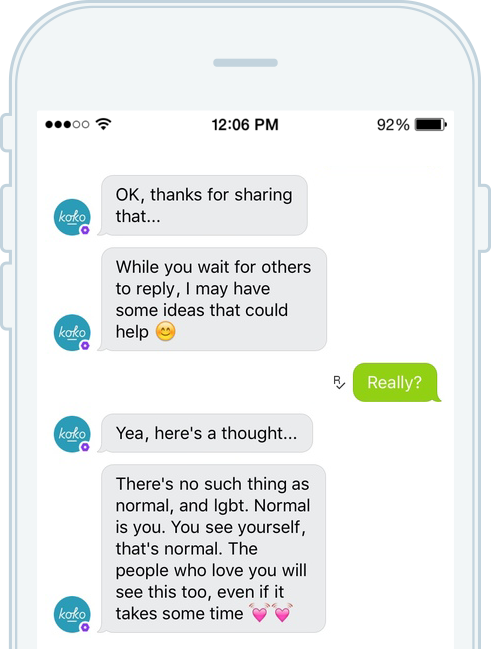
\includegraphics[scale=0.5]{koko_screenshot}
	\caption{Screenshot of the Koko app, obtained from \url{https://www.koko.ai/} on 04/21/2021}
	\label{fig:koko}
\end{figure}
\\
It's important to mention GPT-3 as a whole as well, which, to date, it's one of the most impressive AI algorithm to be developed, the downsides being that it's still in beta phase, it's super resource-heavy, and its access is reserved to businesses through a fee, very expensive to use for the general public, especially students as myself. That's why in this paper, TensorFlow is used, which is free to use, doesn't need a lot of resources to work and it's portable once it's trained.

\clearpage